\subsection{Physical performance with silicon of different thickness} 
\label{sec:physical}

As the known,
the silicon sensors have to work at around $-30^{\circ}\hspace{-0.09em}\mathrm{C}$,
to reliably operate silicon sensors after irradiation,
and to keep low electronic noise causing from leakage current.
The evaporative $\mathrm{CO}_{2}$ is popularly used to cool the silicons sensors,
which go through the pipes in the copper cooling plane
as the copper can provide excellent thermal conductivity.
In order to study the effect to the performance of copper plane cryostat,
we change the geometry to each layer,
with $6\mm$ copper plane added,
which is attached to the silicon sensors.
This is a safe estimation,
usually 26 cooling layers are not necessary,
according to the study from CMS HGCAL group,
five plants are employed to cool the system totally.
The physical performances with copper cryostat are also studied.  


\subsubsection{$\Bs\to\phi\gamma$ performance}
The simulation sample of this decay channel was generated in $\lum=4\times10^{32}\cm^{-2}\cdot\sec^{-1}$ situation,
details procedure is shown in Figure.~\ref{fig:process}.
The reconstruction method for this channel is as same as the one performed in parameterized simulation.  
Figure.~\ref{fig:Bs_mass_B2PhiGamma} presents the mass distributions of \Bs mesons which are constructed in $\Bs\to\phi\gamma$ channel with different thickness of silicon sensor.
It is obvious that the Si-W with copper cooling included leads to a worse \Bs mass resolution.
Besides,
these results are consistent to these obtained from parameterized simulation. 
%It is obvious that the combinatorial background is significantly suppressed with the time requirement.
\begin{figure}[!htbp]
  \begin{center}
    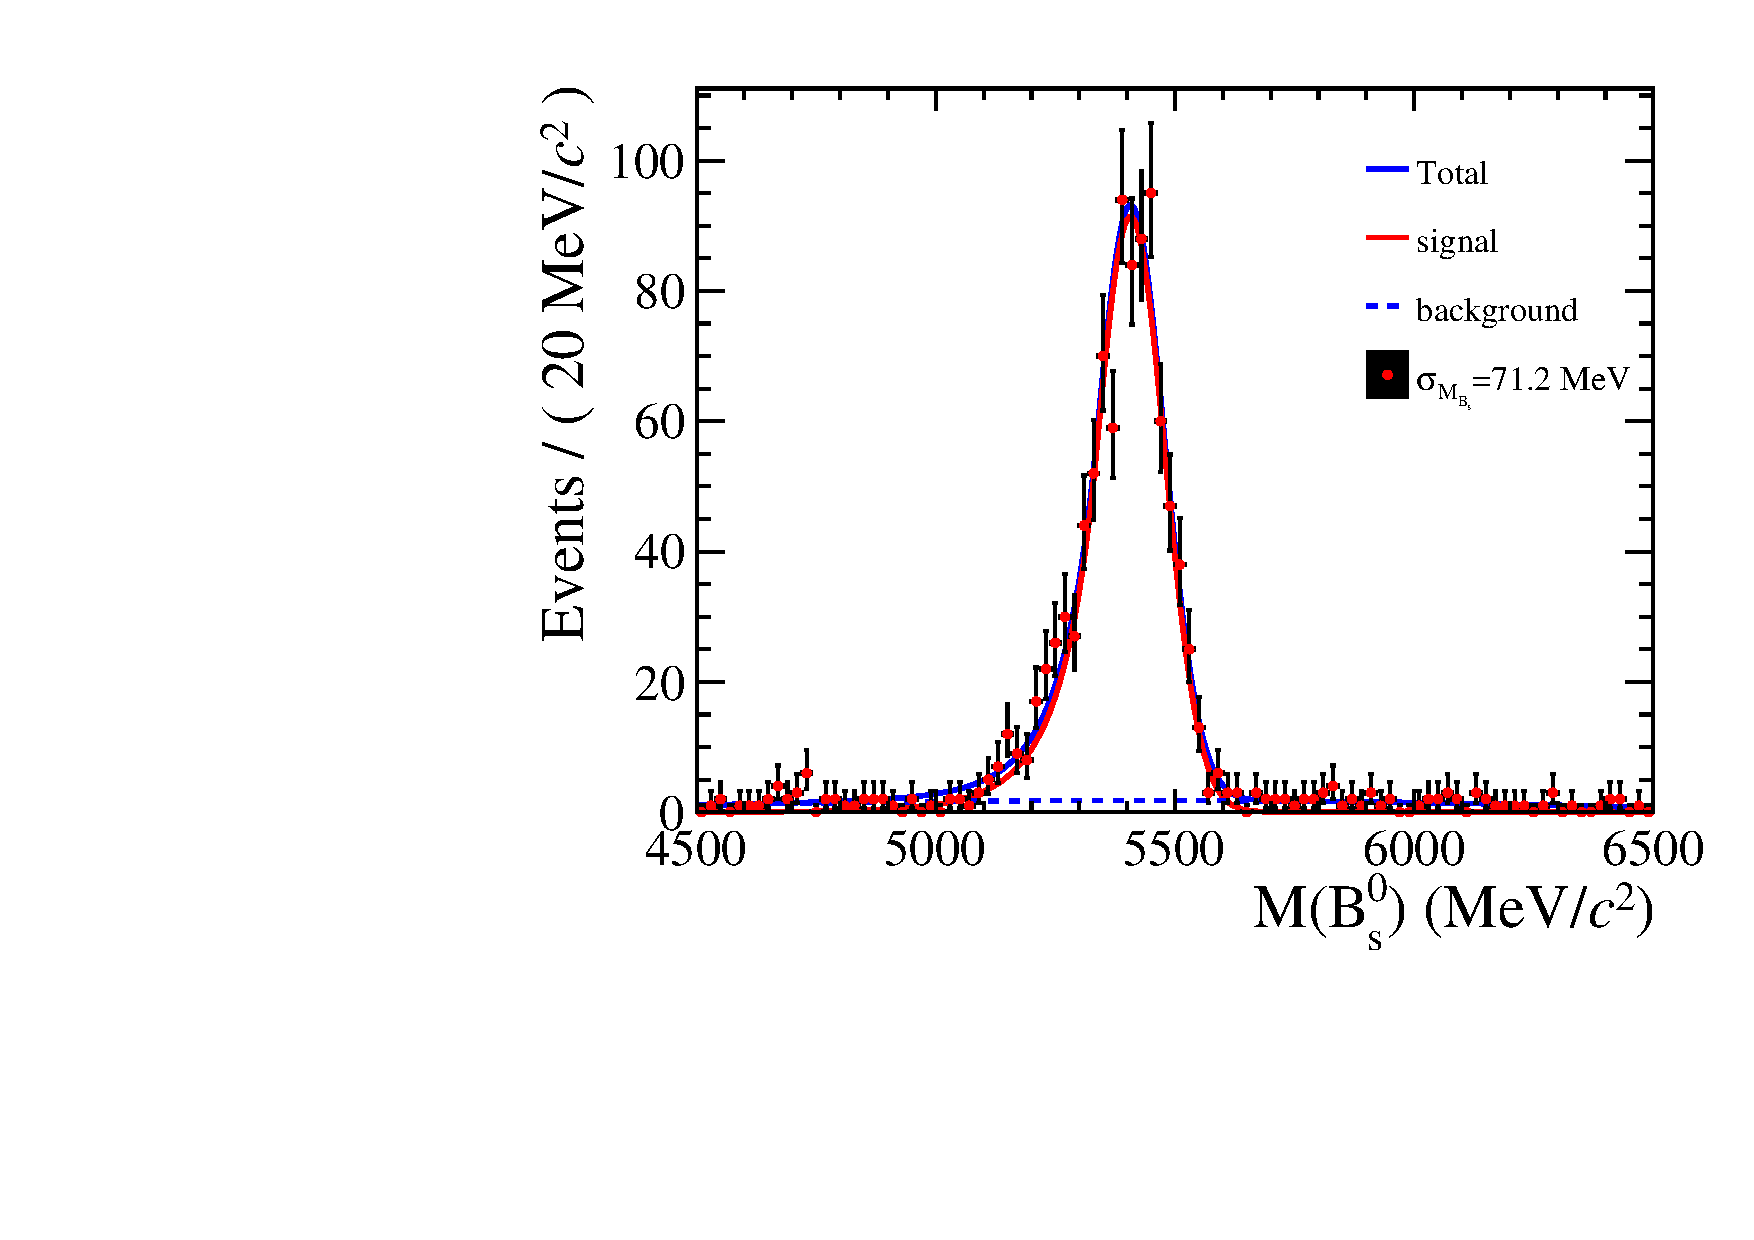
\includegraphics[width=0.49\linewidth]{Figures/06_ECAL/Bs_PhiGamma/diff_thickness/low_lumi/plots/Bs_0_2.pdf}
    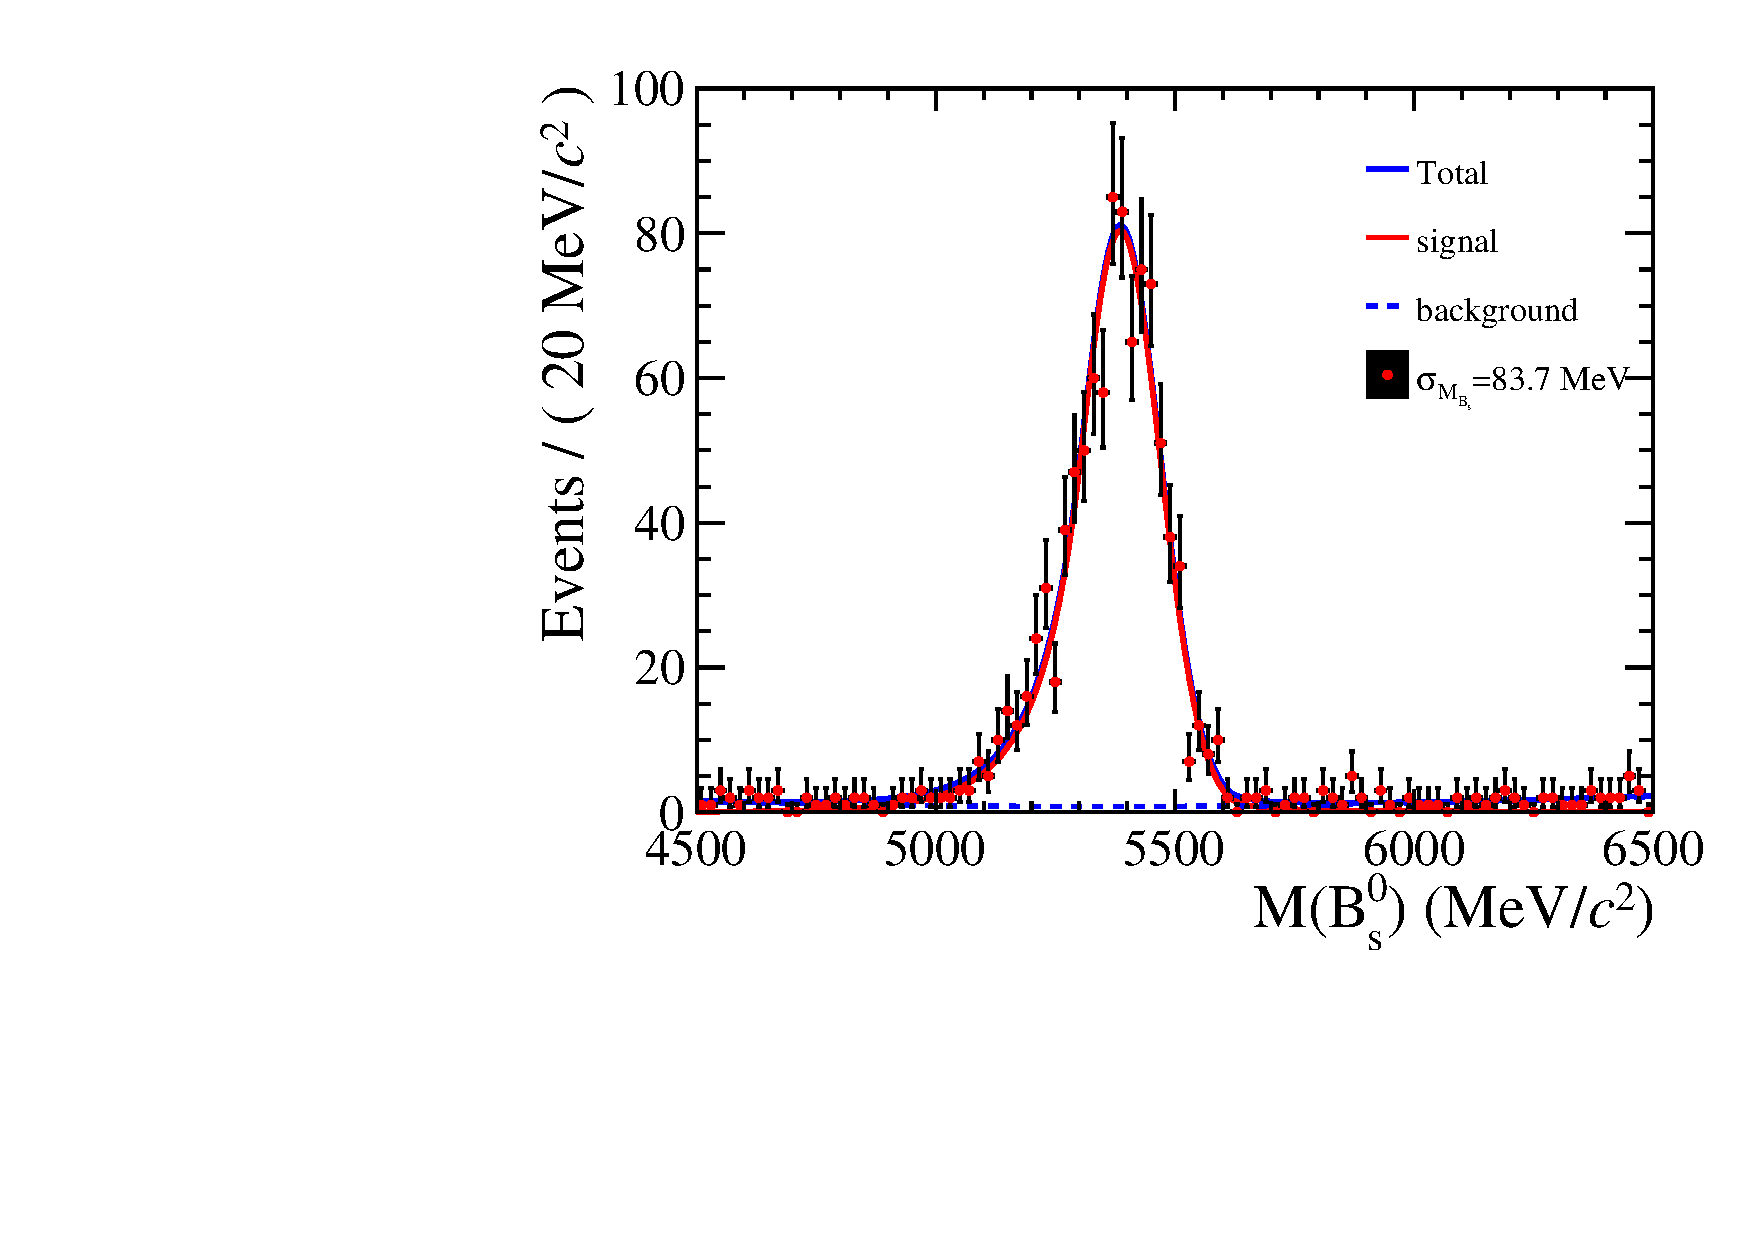
\includegraphics[width=0.49\linewidth]{Figures/06_ECAL/Bs_PhiGamma/diff_thickness/low_lumi/plots/Bs_Cu_0_2.pdf}
    \vspace*{-0.5cm}
  \end{center}
  \caption{
    %\small %captions should be a little bit smaller than main text
   Mass distributions of the $\Bs$ mesons from $\Bs\to\phi\gamma$ decays. 
   The thickness of silicon sensor is $2\mm$, no copper cryostat applied (left). 
   The thickness of silicon sensor is $2\mm$, 26 cooling copper plane added against silicon layers.
  }
  \label{fig:Bs_mass_B2PhiGamma}
\end{figure}
%%%%%%%%%%%%%%%%%%%%%%%%%%

%Figure.~\ref{fig:B2PhiGamma_eff_vs_puri} shows the efficiency versus the purity of the reconstructed $\Bs$ candidates in 3 of layers with time information, 
%whose mark number are 4,5 and 6.

%\begin{figure}[!htbp]
%    \begin{center}
%    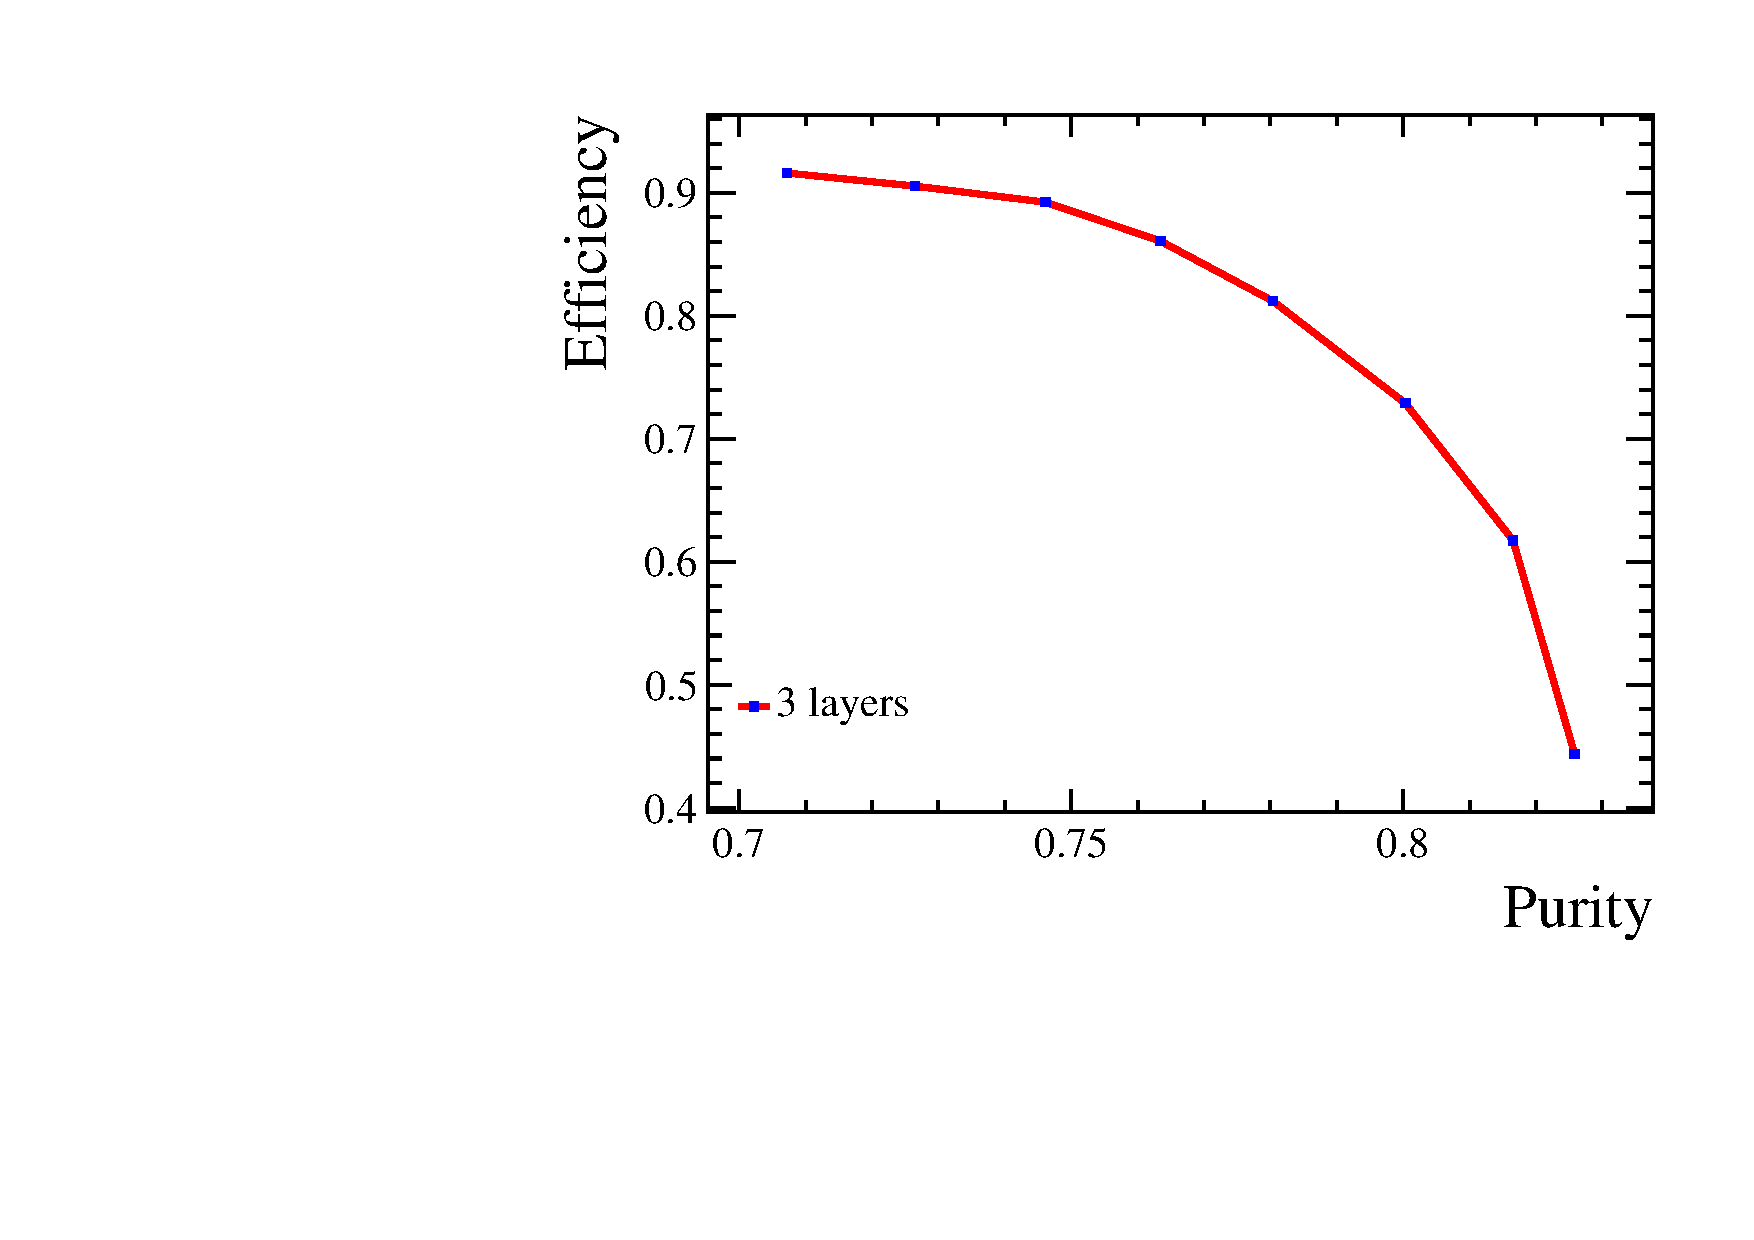
\includegraphics[width=0.49\linewidth]{Figures/06_ECAL/Bs_PhiGamma/Bs_PhiGamma_eff_puri.pdf}
%    \end{center}
%    \caption{Efficiency versus purity of the reconstructed $\Bs$ candidates in 3 of layers in $[5066.89,5666.89]\mev$}
%    \label{fig:B2PhiGamma_eff_vs_puri}
%\end{figure}



\subsubsection{$\Bs\to\jpsi\piz$ performance}

The decay channel $\Bs\to\jpsi\piz$ is used to study the performance for $\piz$ mesons.
Figure~\ref{fig:piz_mass_B2Jpsipiz} shows the mass distributions of the $\piz$ mesons from $\Bs\to\jpsi\piz$ decays.
%The left plot is the mass distribution without the exploitation of any time information. 
%The right plot shows the results with different selections using the time information provided in the simulation. 
%The combinatorial background is significantly suppressed with the time information, 
%\ie $T=T_{\mathrm{arrival}}-\Delta T$ with $\Delta T \equiv (\sqrt{z_{\mathrm{ECAL}}^2+x_{\mathrm{cell}}^2+y_{\mathrm{cell}}^2}-z_{\mathrm{ECAL}})/c$, 
%where $T_{\mathrm{arrival}}$ is the time when the photon arrives at the first layer of the ECAL, 
%$z_{\mathrm{ECAL}}$ is the $z$-coordinate of the first layer of the ECAL, 
%and $x_{\mathrm{cell}}$ ($y_{\mathrm{cell}}$) is the $x$- ($y$-)coordinate of the cell that the shower starts.
%The first beam tests results of the prototype silicon modules for the CMS HGCAL show that a precision of better than $20\ps$ was achieved for $(S/N)_{\mathrm{eff}}>100$\cite{Akchurin:2018rpm}. 
%With a selection of $T<20\ps$, the signal-background ratio looks quite promising.
%The efficiency of the selection of $T<20\ps$ is around $xxx$, and the signal-background ratio is around $xxx$.
%%%%%%%%%%%%%%%%%%%%%%%%%%%%%%%%%%%%%%%%
\begin{figure}[!htbp]
  \begin{center}
    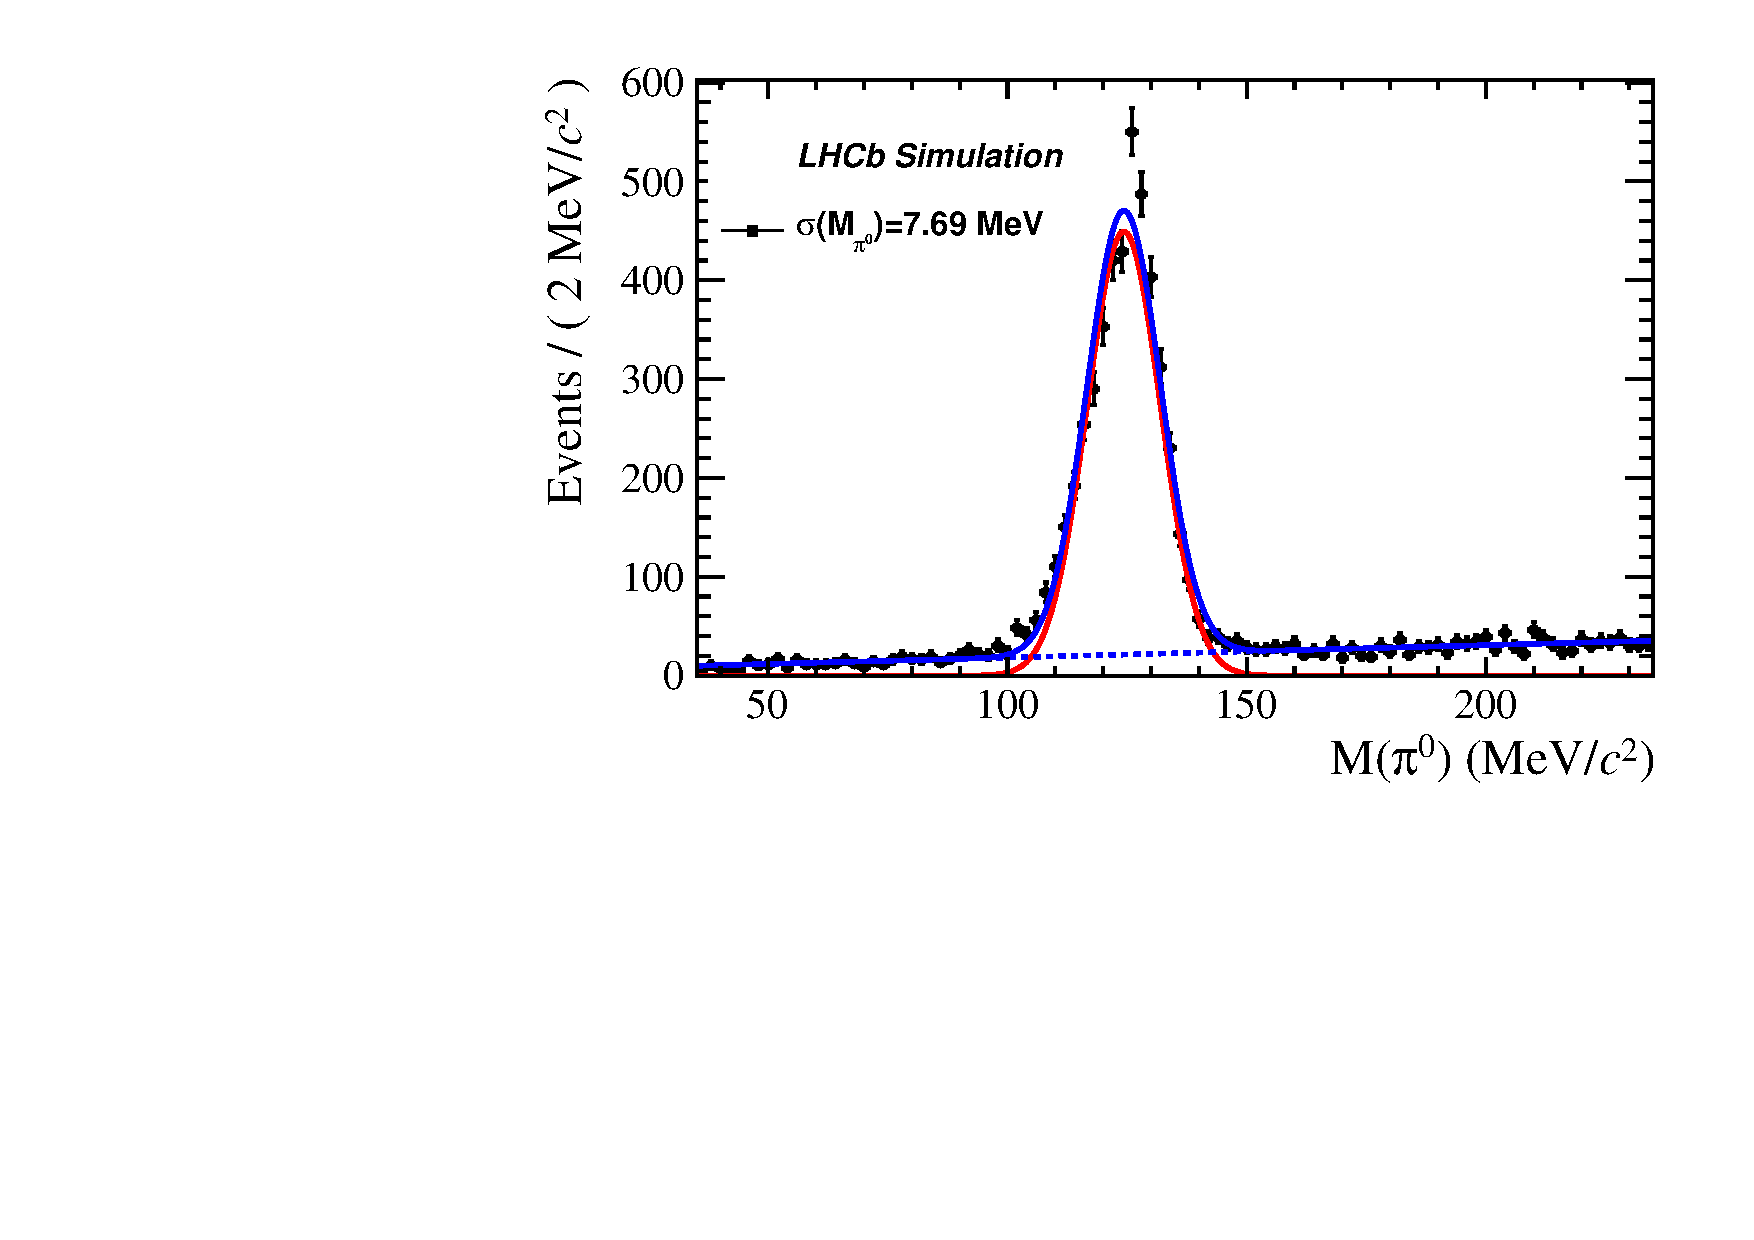
\includegraphics[width=0.49\linewidth]{Figures/06_ECAL/Bs_JpsiPi0/Bs_JpsiPiz/low_lumi/0_2/pi0_M.pdf}
    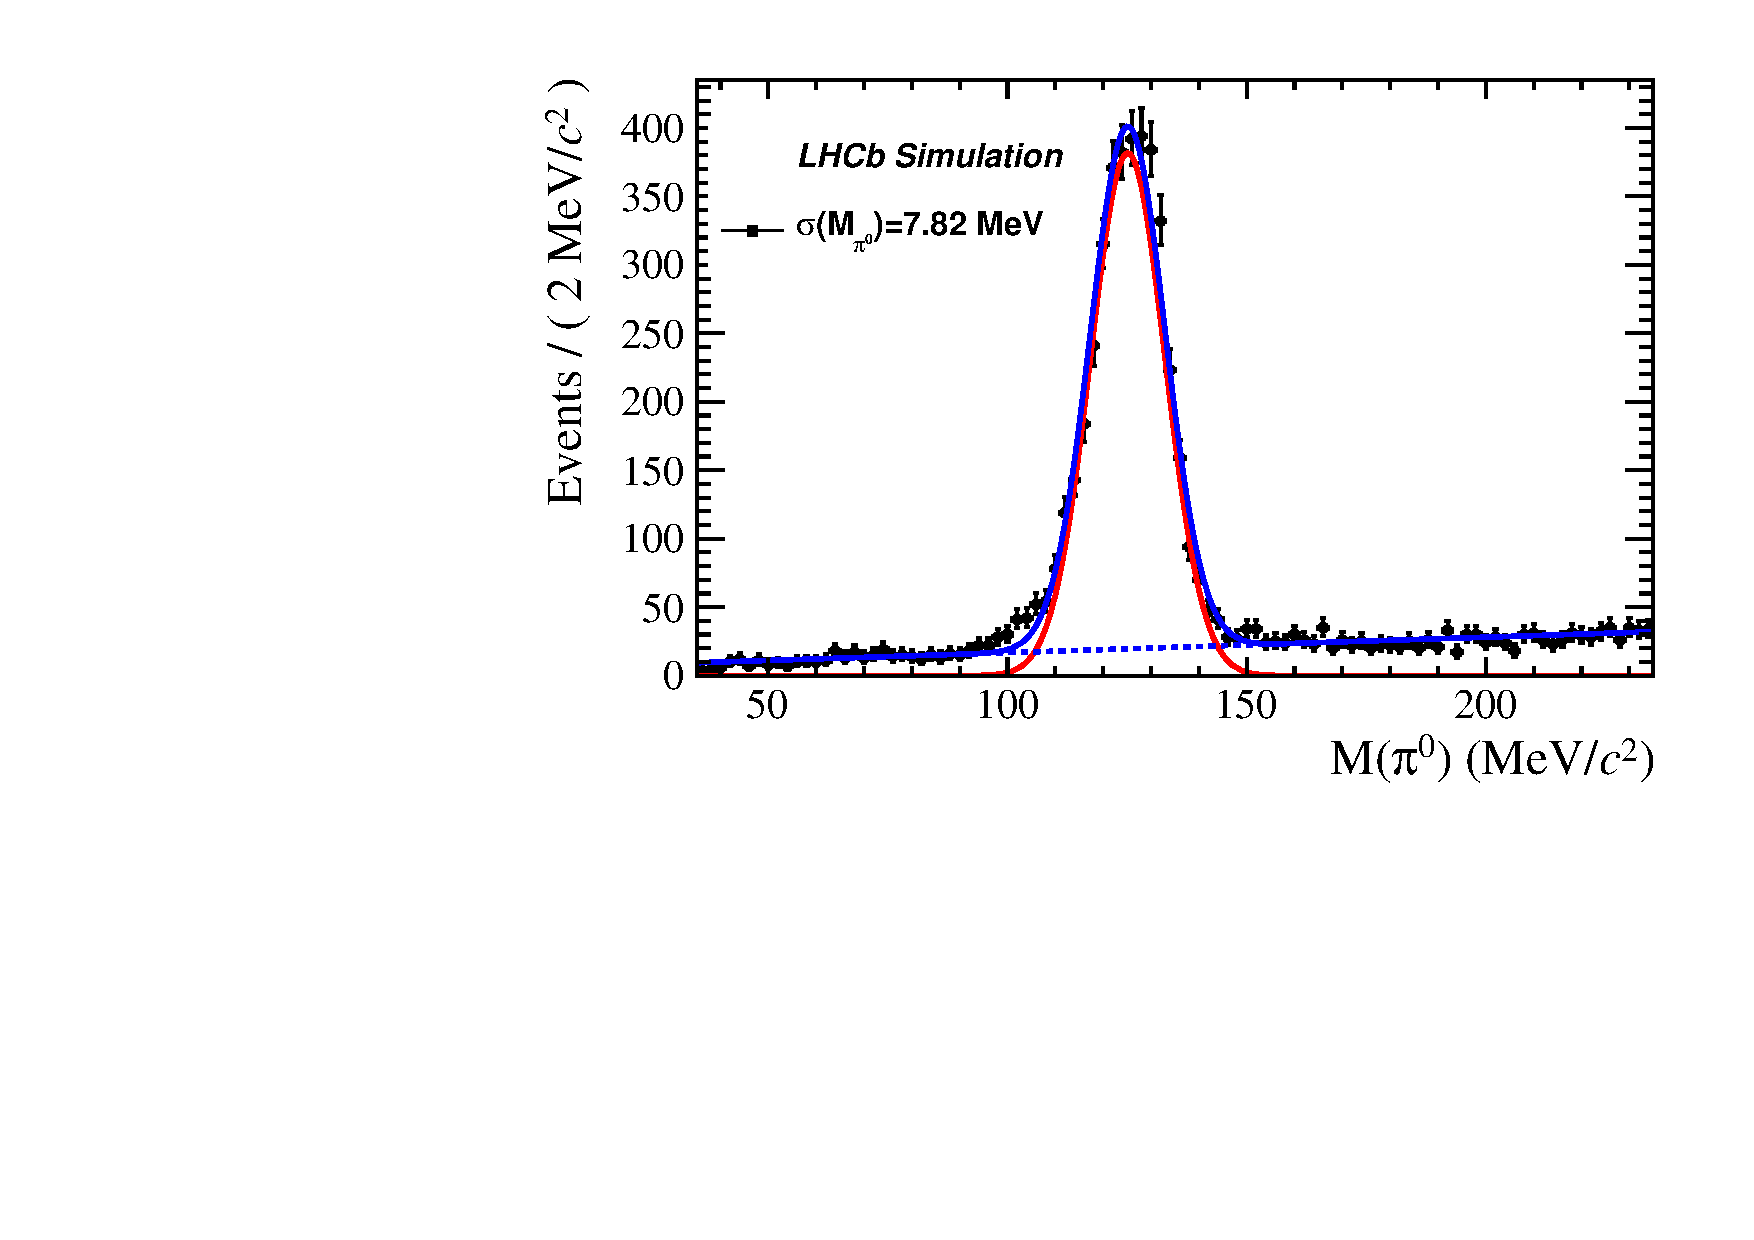
\includegraphics[width=0.49\linewidth]{Figures/06_ECAL/Bs_JpsiPi0/Bs_JpsiPiz/low_lumi/Cu_0_2/pi0_M.pdf}
    \vspace*{-0.5cm}
  \end{center}
  \caption{
    %\small %captions should be a little bit smaller than main text
      Mass distributions of the $\piz$ mesons from $\Bs\to\jpsi\piz$ decays. 
      The thickness of silicon sensor is $2\mm$, no copper cryostat applied (left). 
      The thickness of silicon sensor is $2\mm$, 26 cooling copper plane added against silicon layers.
  }
  \label{fig:piz_mass_B2Jpsipiz}
\end{figure}
%%%%%%%%%%%%%%%%%%%%%%%%%%%%%%%%%%%%%%%%
Besides,
the $\Bs$ mass resolution is also studied.
Figure.~\ref{fig:Bs_Jpsipi0} shows the $\Bs$ mass distributions with $\lum=4\times10^{32}\cm^{-2}\cdot\sec^{-1}$.
The left one is the result with the thickness of silicon sensor equal to $2\mm$,
while the right one shows the result with copper cooling plane applied.
Similarly,
the results from \geant simulation are consistent to the parameterized simulation conclusion.
%%%%%%%%%%%%%%%%%%%%%%%%%%%%%%%%%%%%%%%%
\begin{figure}[hb]
  \begin{center}
    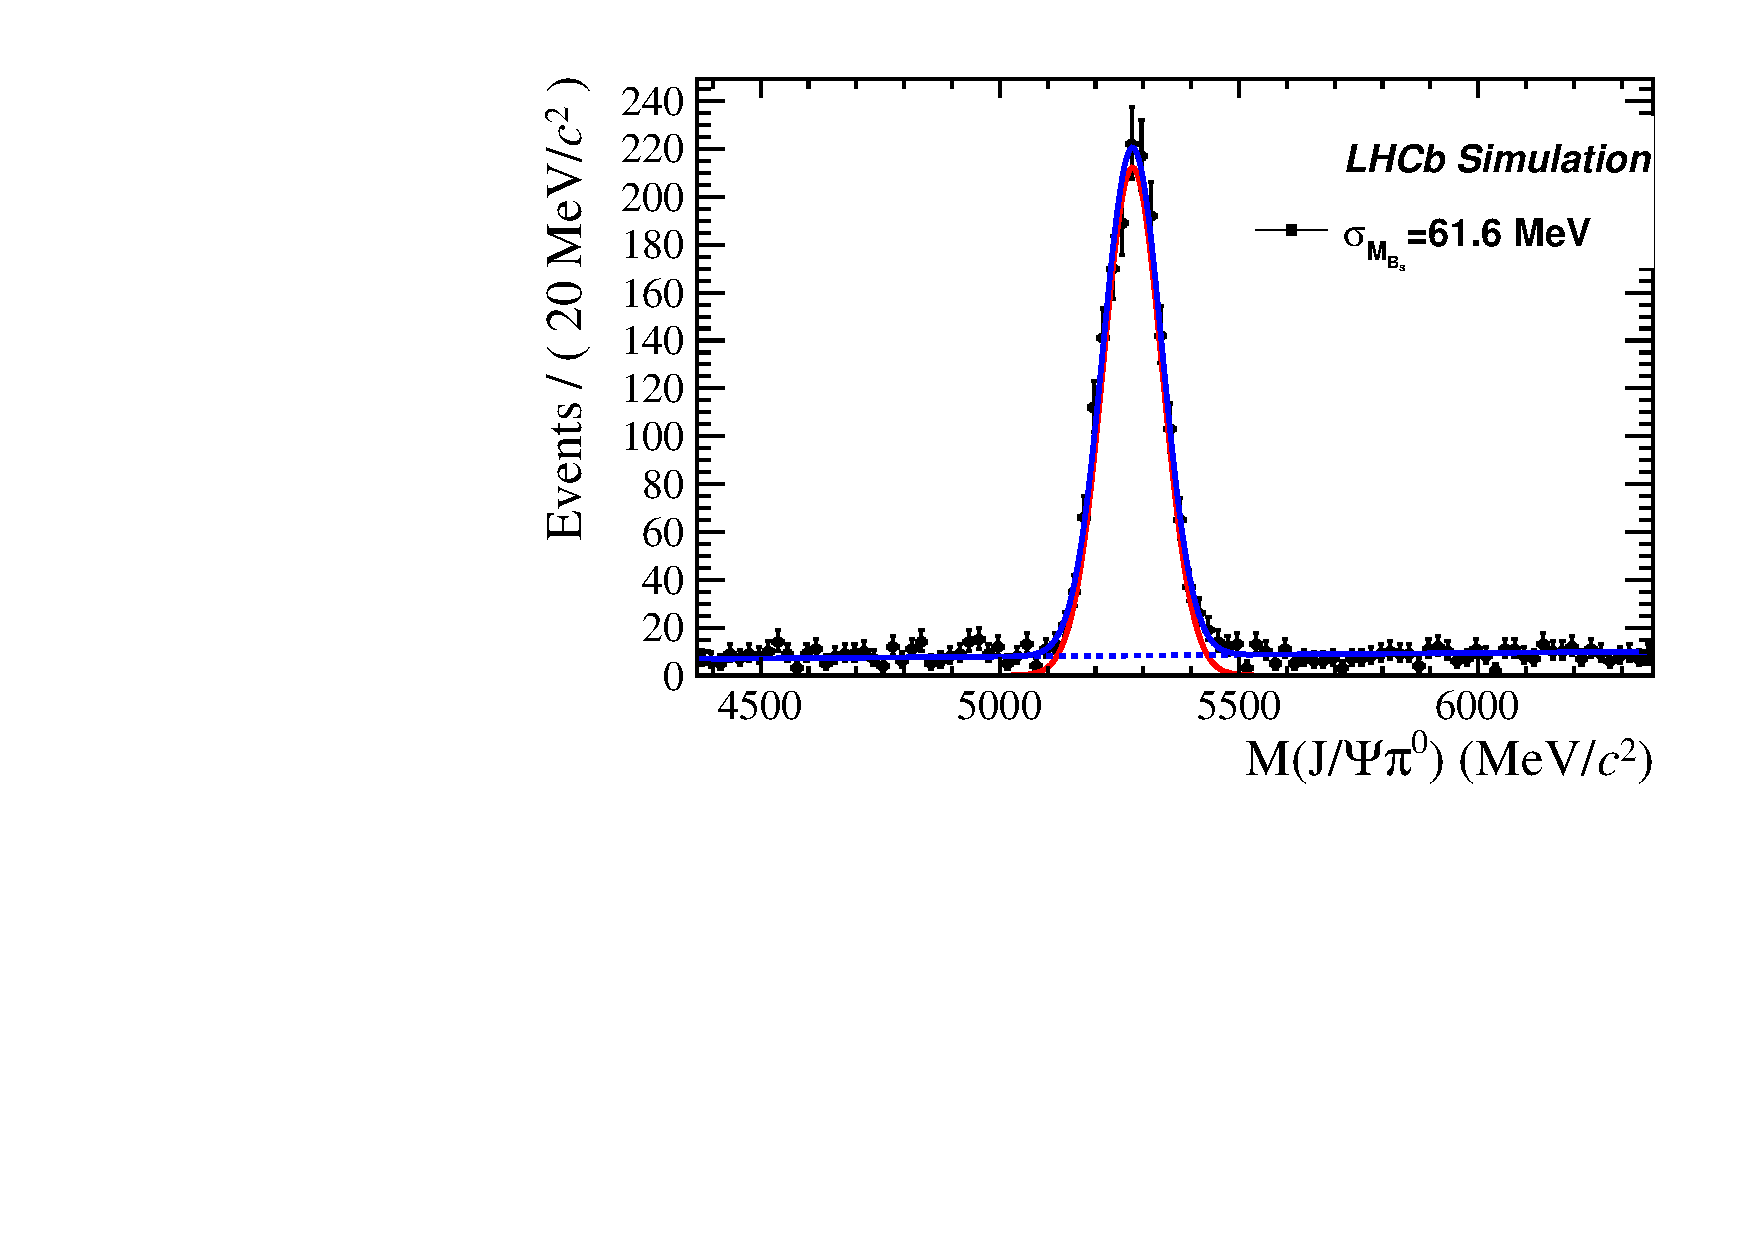
\includegraphics[width=0.49\linewidth]{Figures/06_ECAL/Bs_JpsiPi0/Bs_JpsiPiz/low_lumi/0_2/Bs_JpsiPi0.pdf}
    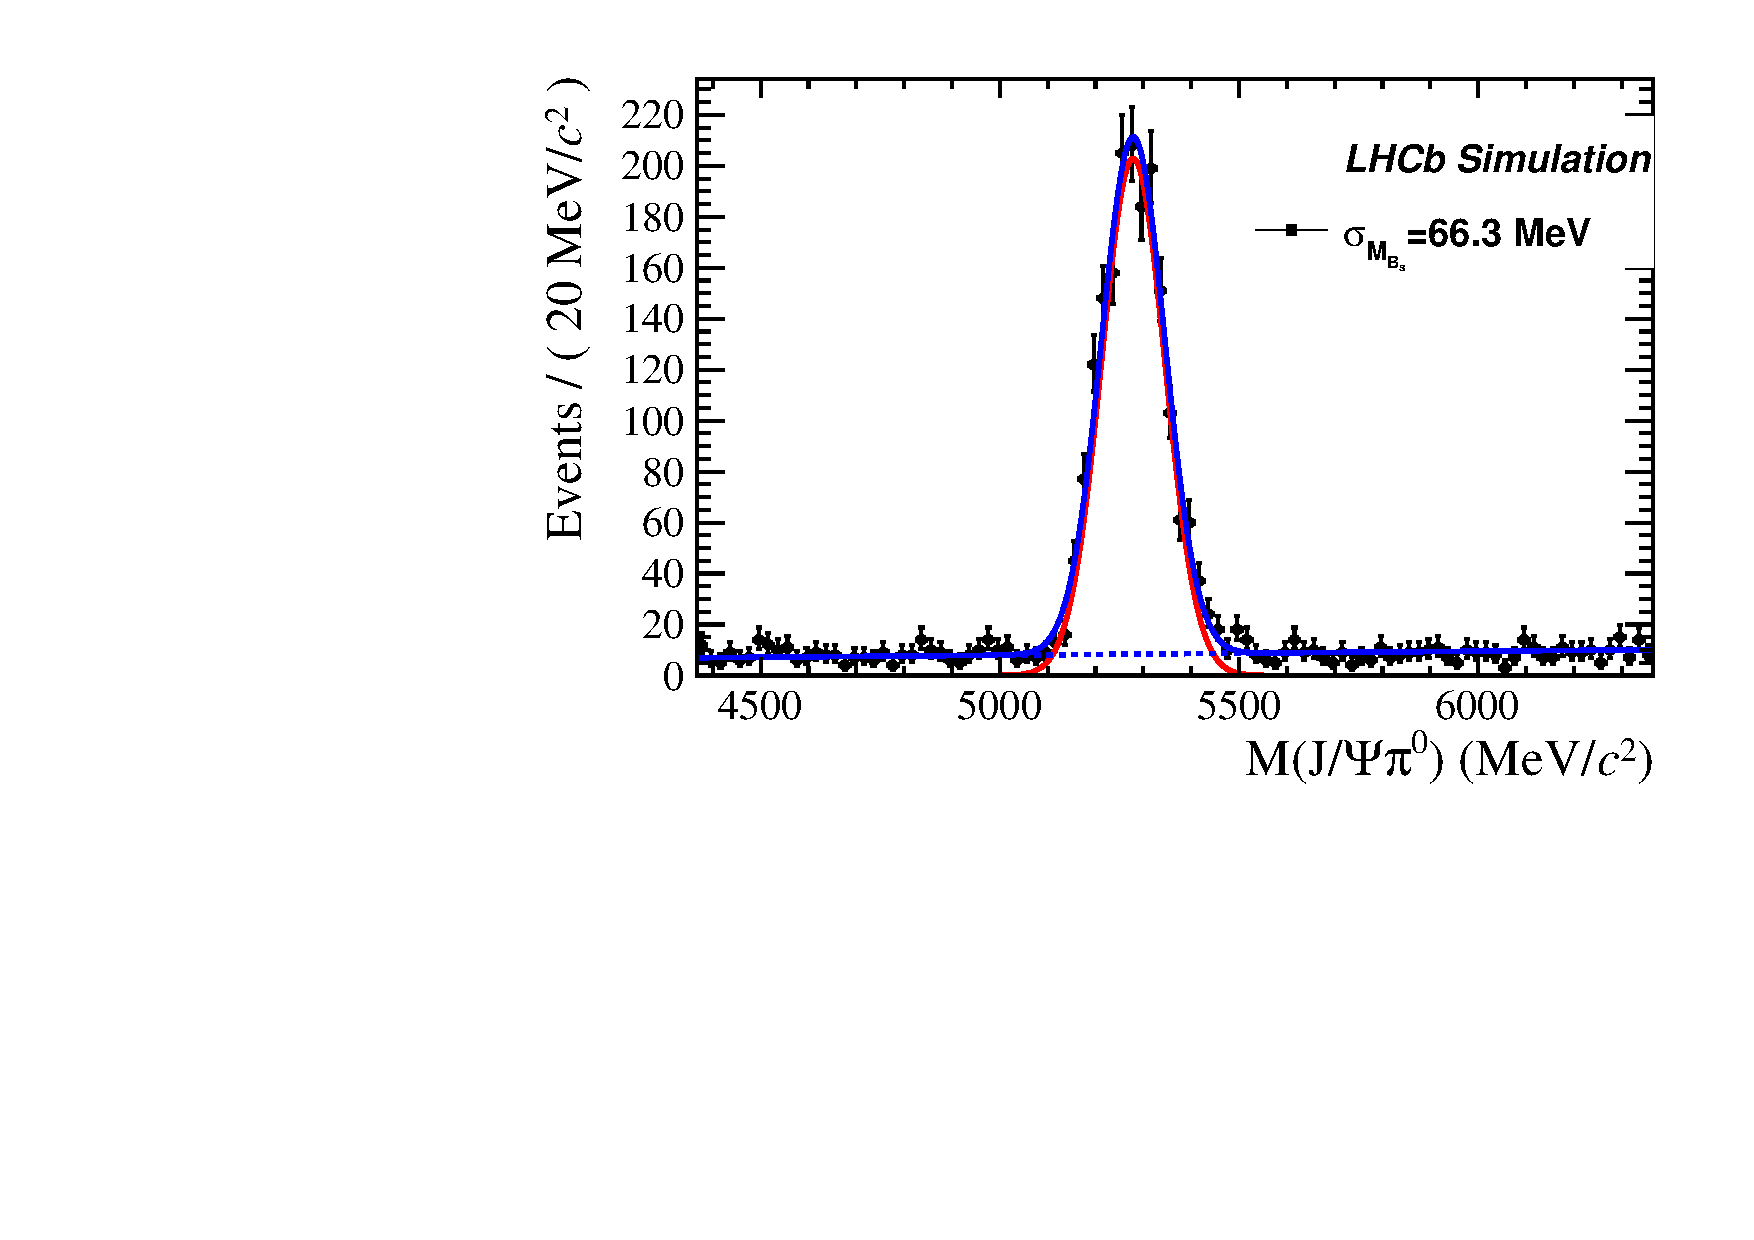
\includegraphics[width=0.49\linewidth]{Figures/06_ECAL/Bs_JpsiPi0/Bs_JpsiPiz/low_lumi/Cu_0_2/Bs_JpsiPi0.pdf}
    \vspace*{-0.5cm}
  \end{center}
  \caption{
      The $\Bs$ mass distribution reconstructed from $\Bs\to\jpsi\piz$ decay. 
      The thickness of silicon sensor is $2\mm$, no copper cryostat applied (left). 
      The thickness of silicon sensor is $2\mm$, 26 cooling copper plane added against silicon layers.
  }
  \label{fig:Bs_Jpsipi0}
\end{figure}
%%%%%%%%%%%%%%%%%%%%%%%%%%%%%%%%%%%%%%%%


%The left plot of Fig.~\ref{fig:timecut} shows the time resolution as a function of the electron energy for the SiW ECAL with six layers that provide time information. The resolution is around $30\ps$ for low energy electrons and is around $10\ps$ for high energy electrons.
%Figure.~\ref{fig:timecut} shows the efficiency versus the purity of the reconstructed $\Bs$ candidates for different numbers of layers with time information. 
%When the number of time layers increases from two to four, the performance improves significantly.
%%%%%%%%%%%%%%%%%%%%%%%%%%%%%%%%%%%%%%%%%
%\begin{figure}[!htbp]
%  \begin{center}
%    %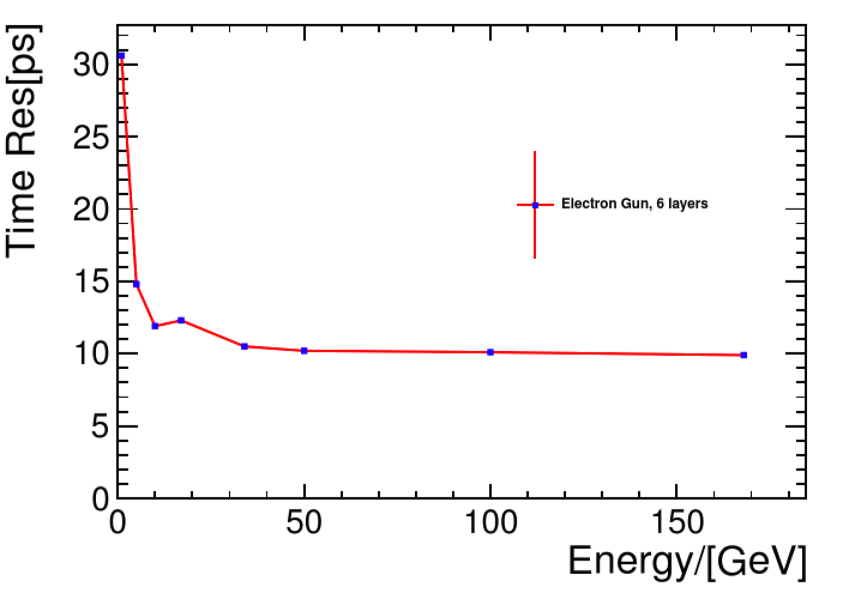
\includegraphics[width=0.49\linewidth]{plotsZW/timeresolution_energy.pdf}
%    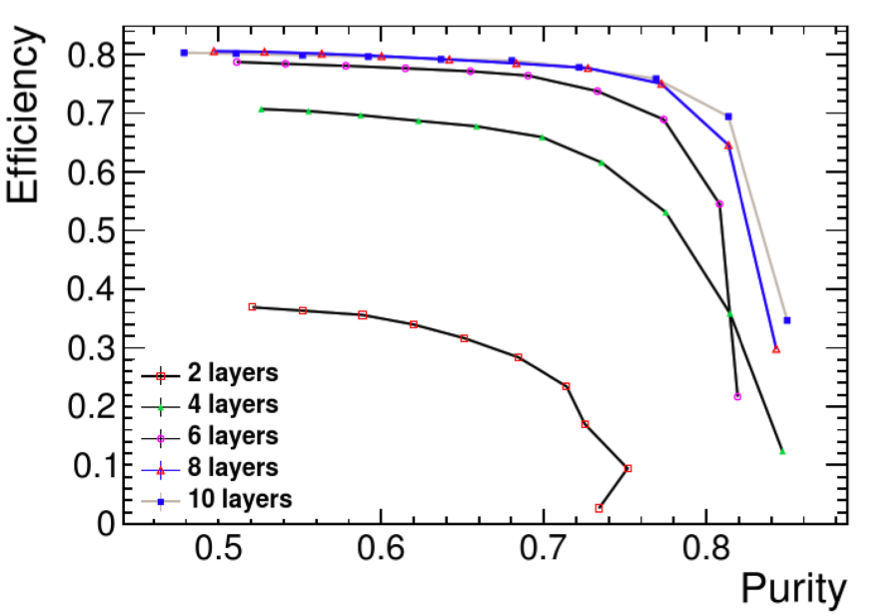
\includegraphics[width=0.49\linewidth]{Figures/06_ECAL/plotsZW/timecut_purity_efficiency.pdf}
%    \vspace*{-0.5cm}
%  \end{center}
%  \caption{
%    %\small %captions should be a little bit smaller than main text
%     %Left: Time resolution as a function of the electron energy for the SiW ECAL with six time layers.
%     Efficiency versus purity of the reconstructed $\Bs$ candidates for different numbers of time layers.
%  }
%  \label{fig:timecut}
%\end{figure}
%%%%%%%%%%%%%%%%%%%%%%%%%%%%%%%%%%%%%%%%%



\subsection{Bremsstrahlung recovery and $\Bd\to\Kstar\en\ep$ performance}

In consideration of the detector material budget before the \ecal,
the electron has possibility to interact with trackers from bremsstrahlung,
which cause the energy measurement to electron is not accurate,
especially the reaction happening before the magnet.
In this case, 
we want to study the method to recover the electron energy by adding the radiated $\gamma$.

The decay channel $\Bd\to\Kstar\en\ep$ is taken as a bechmark channel,
which can be used to study the bremsstrahlung effect.
The electron energy and transverse momentum distribution are shown in Figure.~\ref{fig:Brem_electron_E}.

%%%%%%%%%%%%%%%%%%%%%%%%%%%%%%%%%%%%%%%%
\begin{figure}[!htbp]
  \begin{center}
    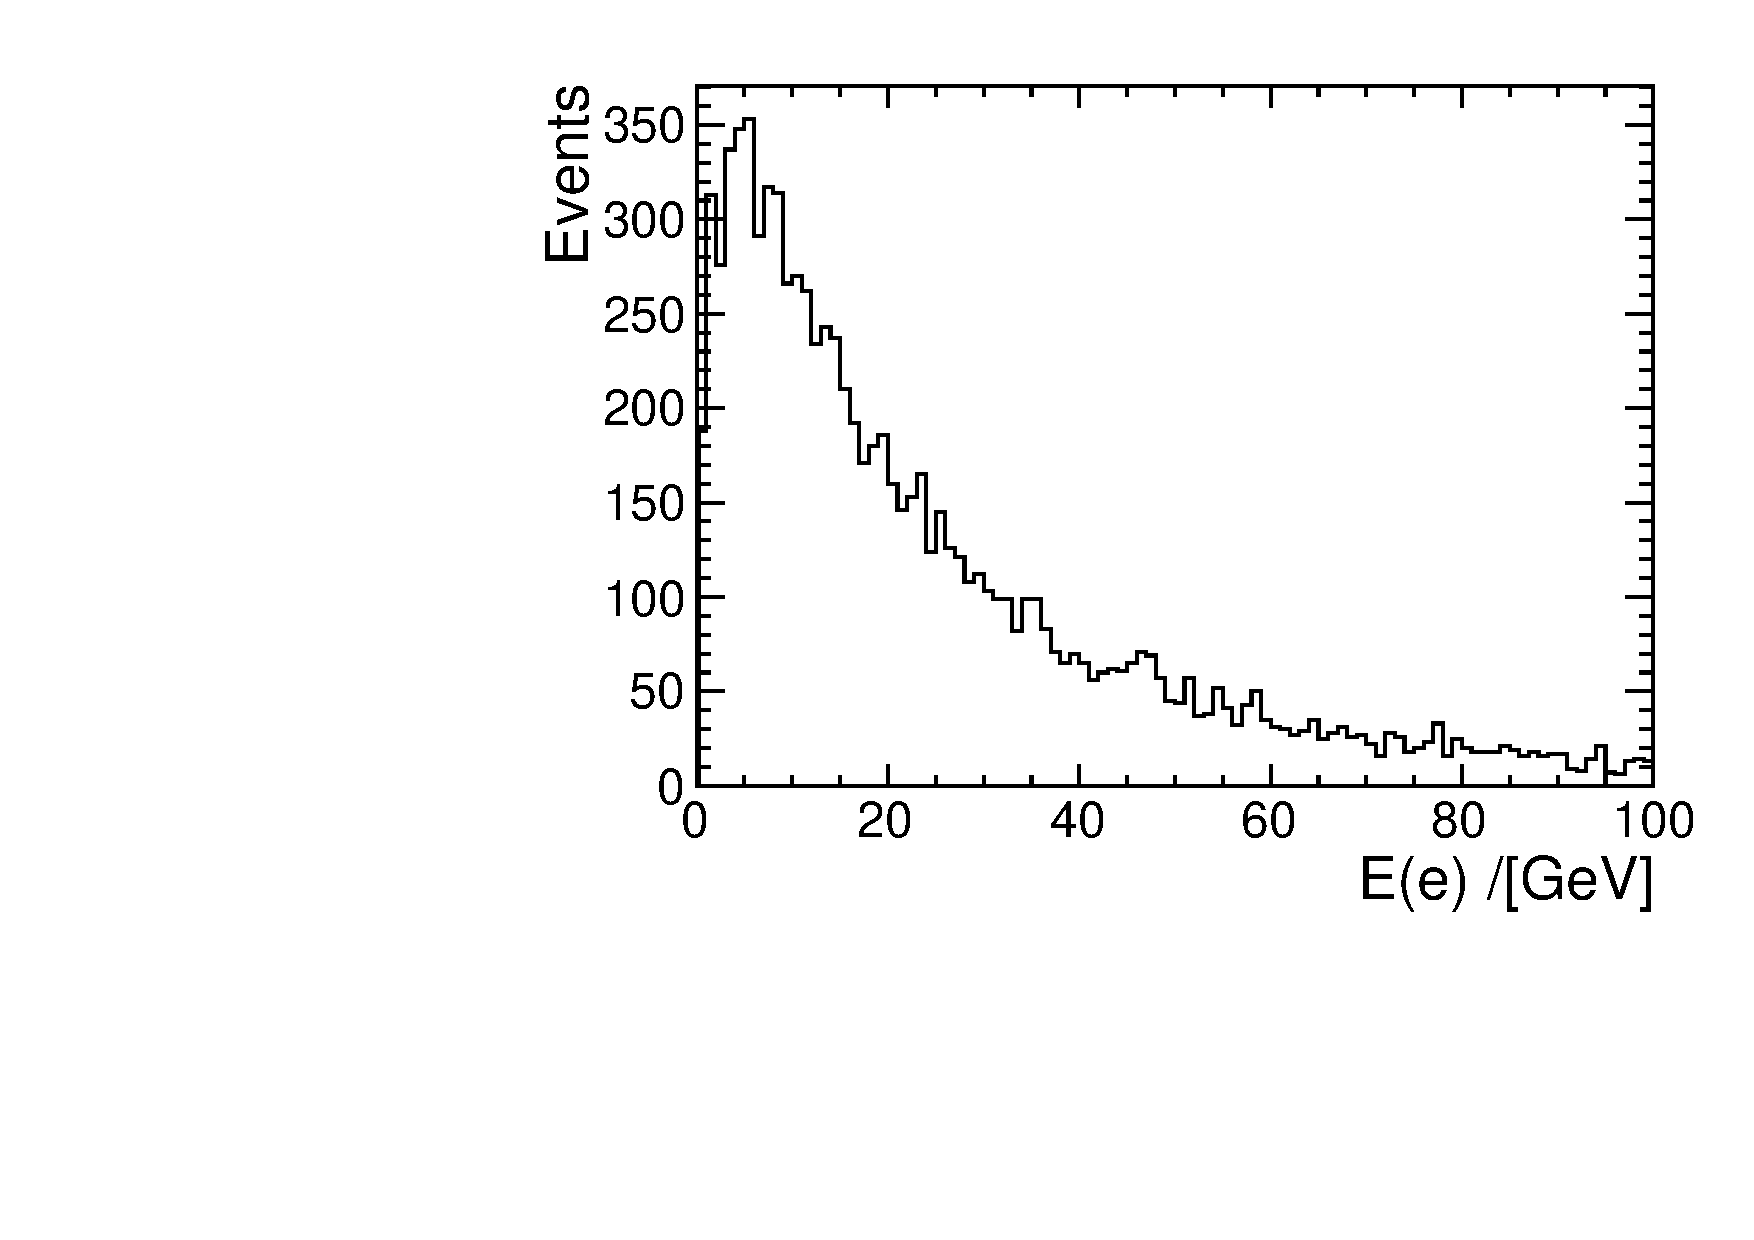
\includegraphics[width=0.49\linewidth]{Figures/06_ECAL/Brem/Electron_E.pdf}
    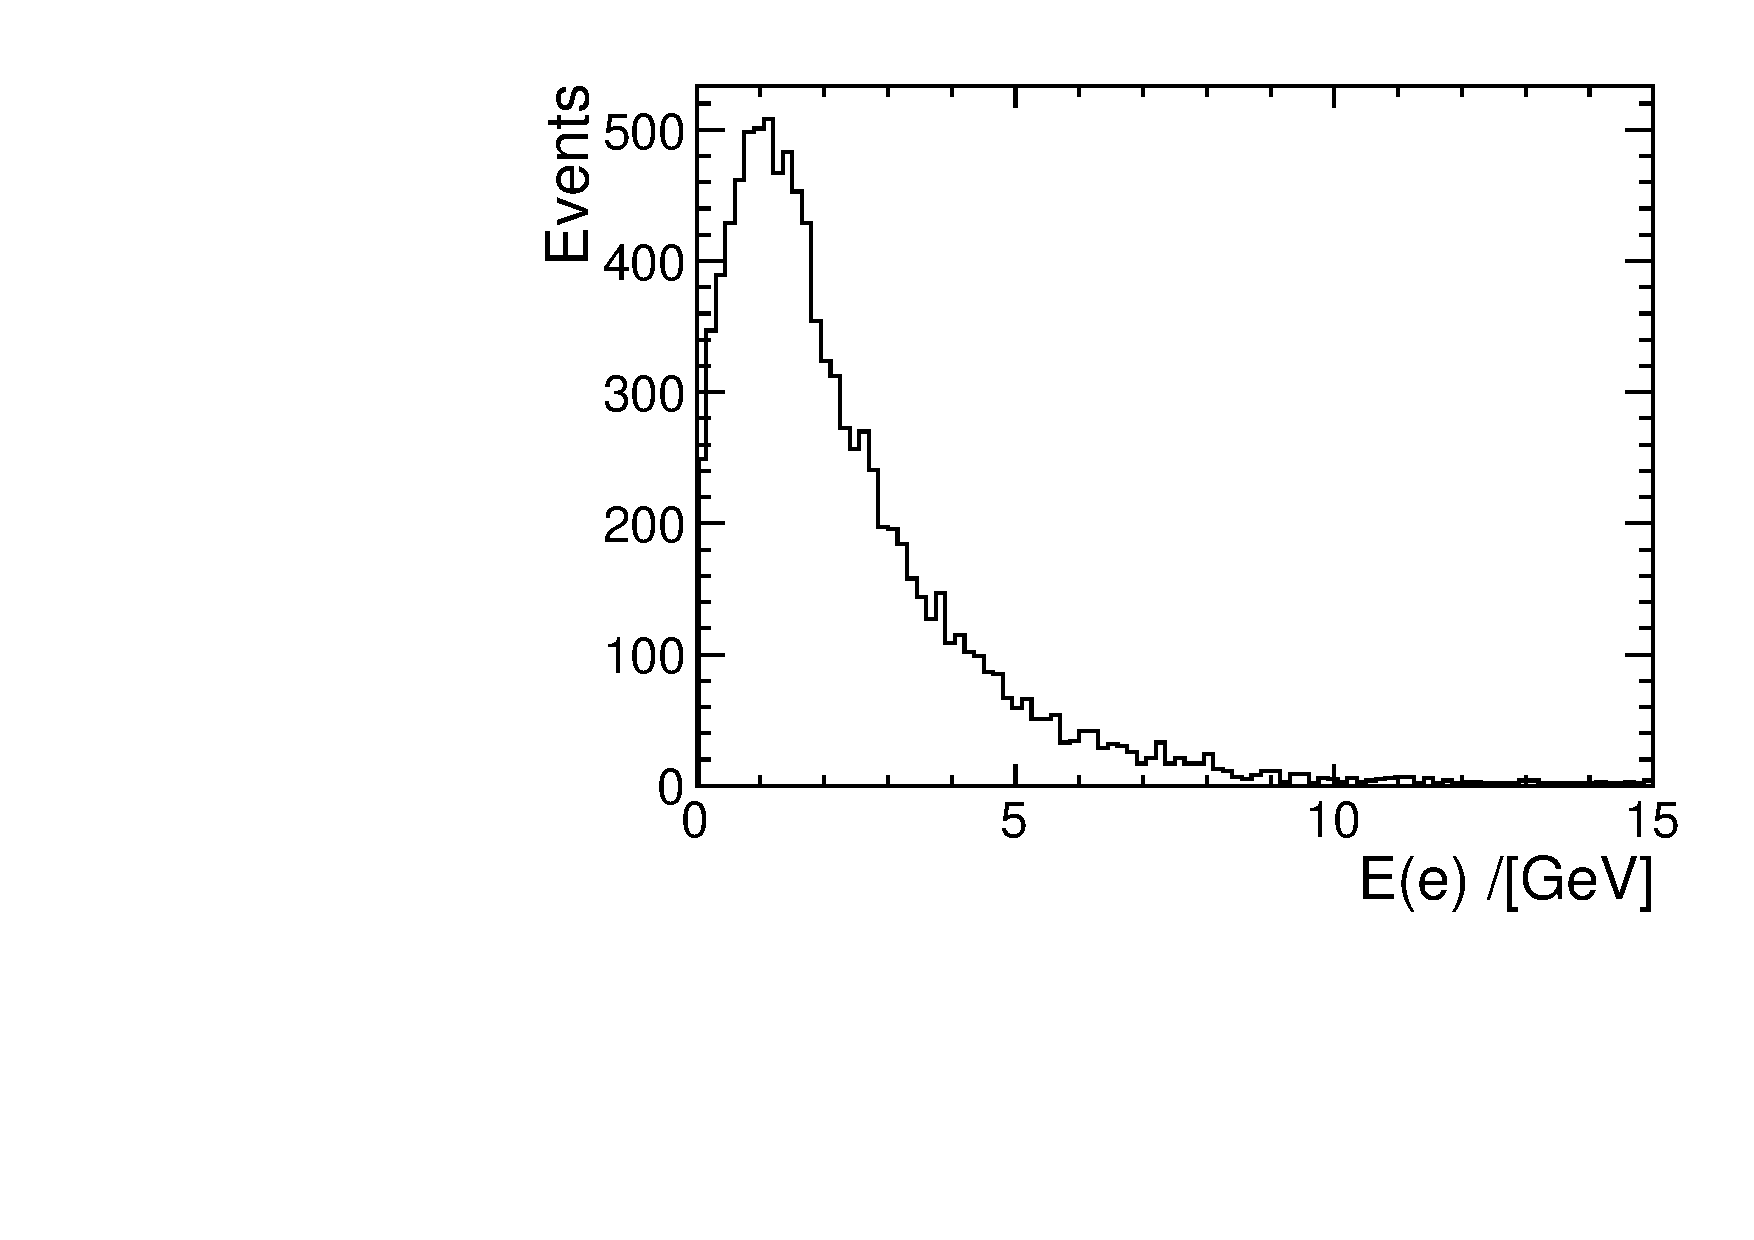
\includegraphics[width=0.49\linewidth]{Figures/06_ECAL/Brem/Electron_PT.pdf}
    \vspace*{-0.5cm}
  \end{center}
  \caption{
      The electron energy(left) and transverse momentum(right) distribution in $\Bd\to\Kstar\en\ep$ decay.
  }
  \label{fig:Brem_electron_E}
\end{figure}
%%%%%%%%%%%%%%%%%%%%%%%%%%%%%%%%%%%%%%%%

We take a look at the distance between the electron and the bremsstrahlung photon on the \ecal plane,
as shown in the Figure.~\ref{fig:Brem_electron_distance}.

%%%%%%%%%%%%%%%%%%%%%%%%%%%%%%%%%%%%%%%%
\begin{figure}[!htbp]
  \begin{center}
    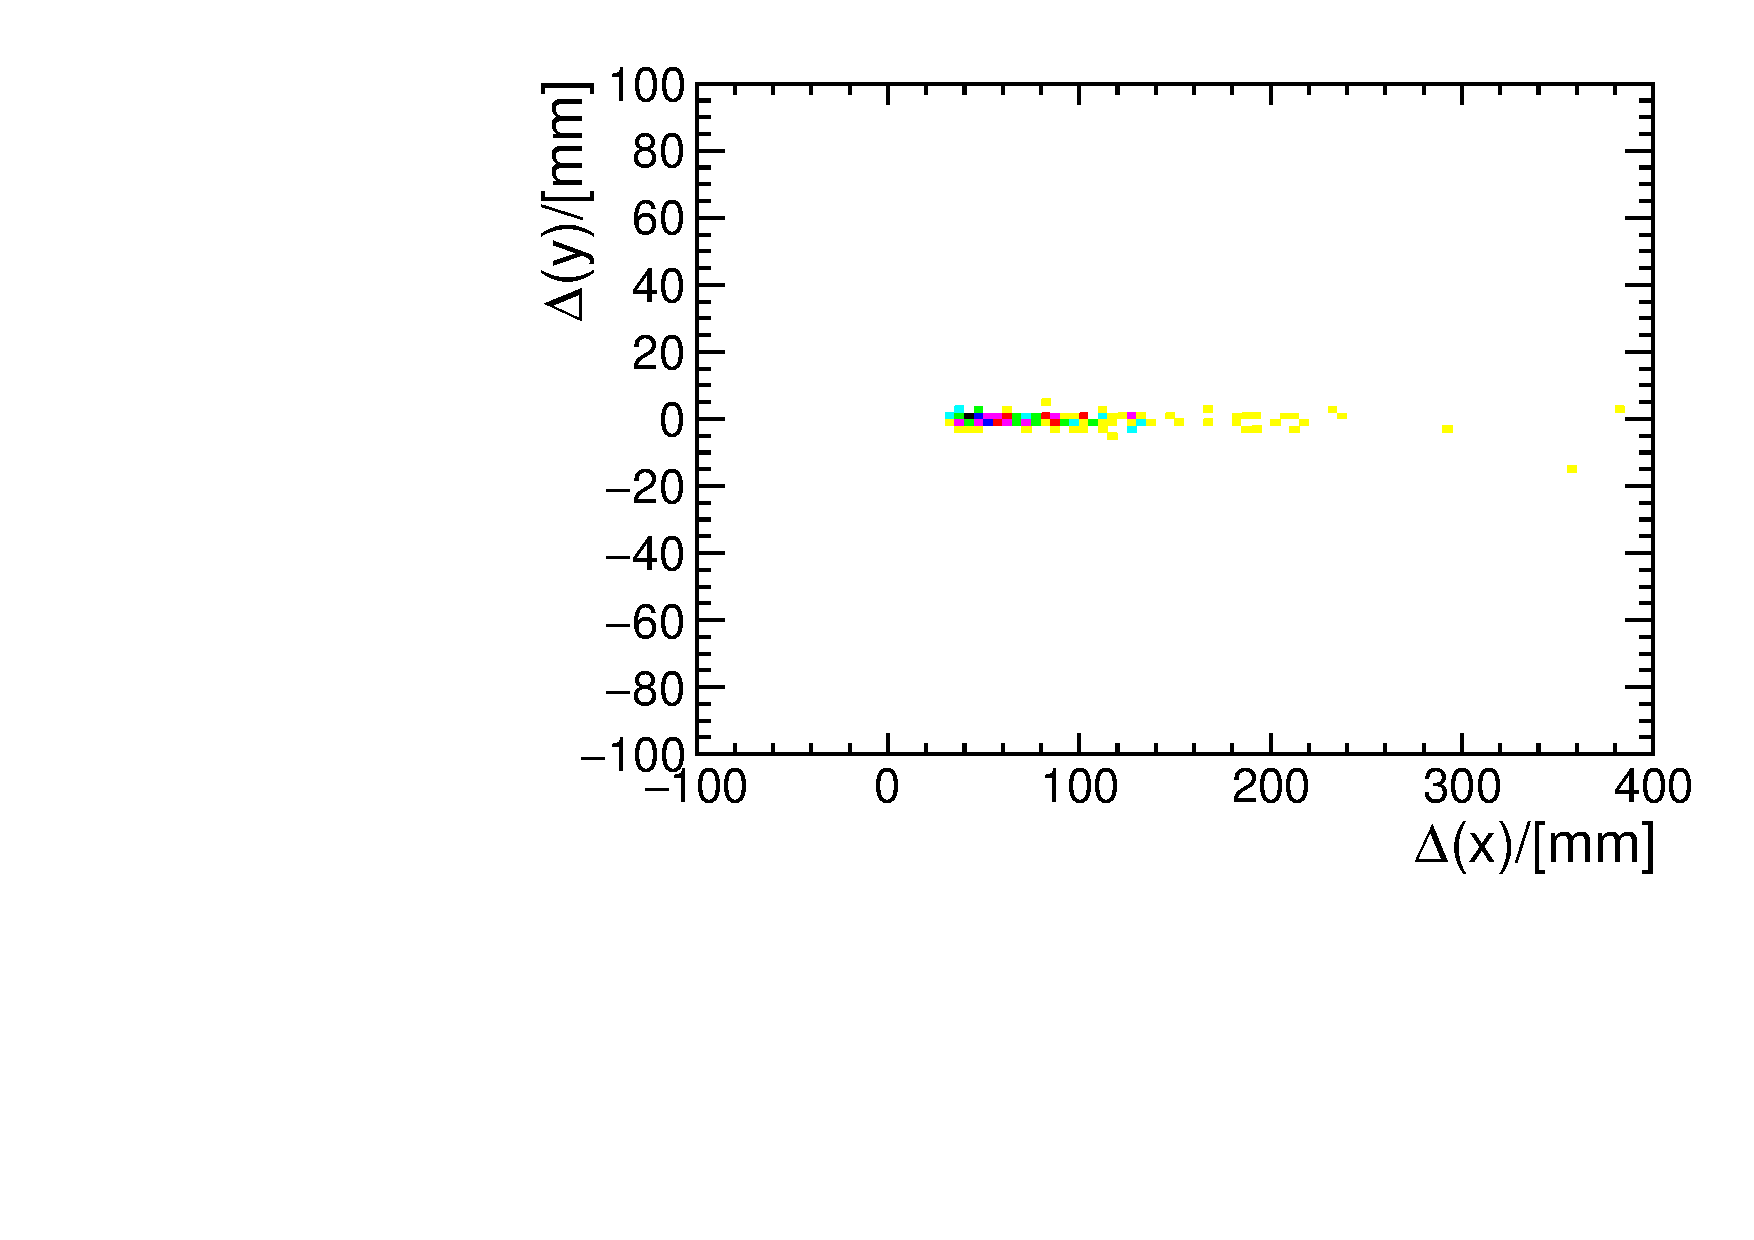
\includegraphics[width=0.49\linewidth]{Figures/06_ECAL/Brem/x_y_dis.pdf}
    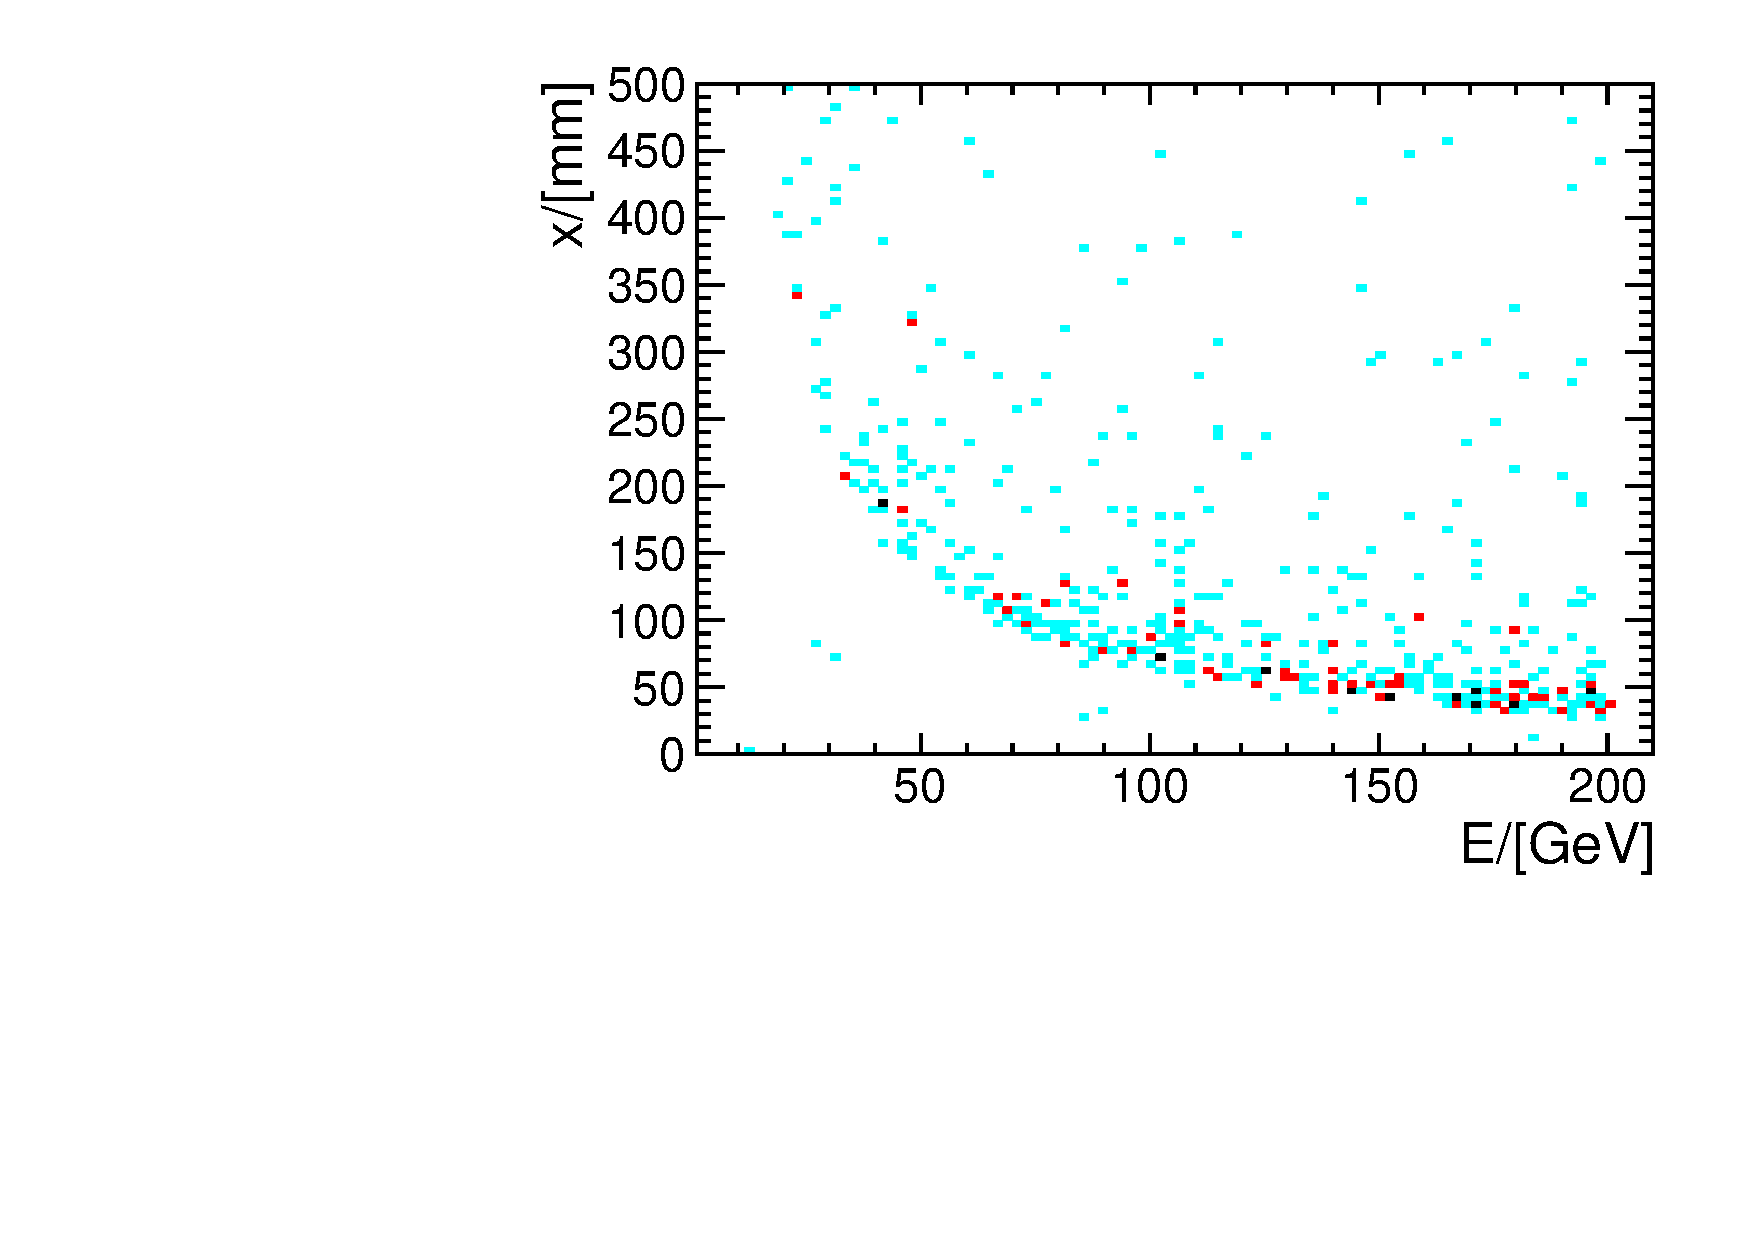
\includegraphics[width=0.49\linewidth]{Figures/06_ECAL/Brem/x_E_dis.pdf}
    \vspace*{-0.5cm}
  \end{center}
  \caption{
  Left: the distance between the electron and bremsstrahlung photon on the \ecal plane; 
  Right: the relation between the electron energy and the x distance on the \ecal plane.
  }
  \label{fig:Brem_electron_distance}
\end{figure}
%%%%%%%%%%%%%%%%%%%%%%%%%%%%%%%%%%%%%%%%

%%%%%%%%%%%%%%%%%%%%%%%%%%%%%%%%%%%%%%%%
\begin{figure}[!htbp]
  \begin{center}
    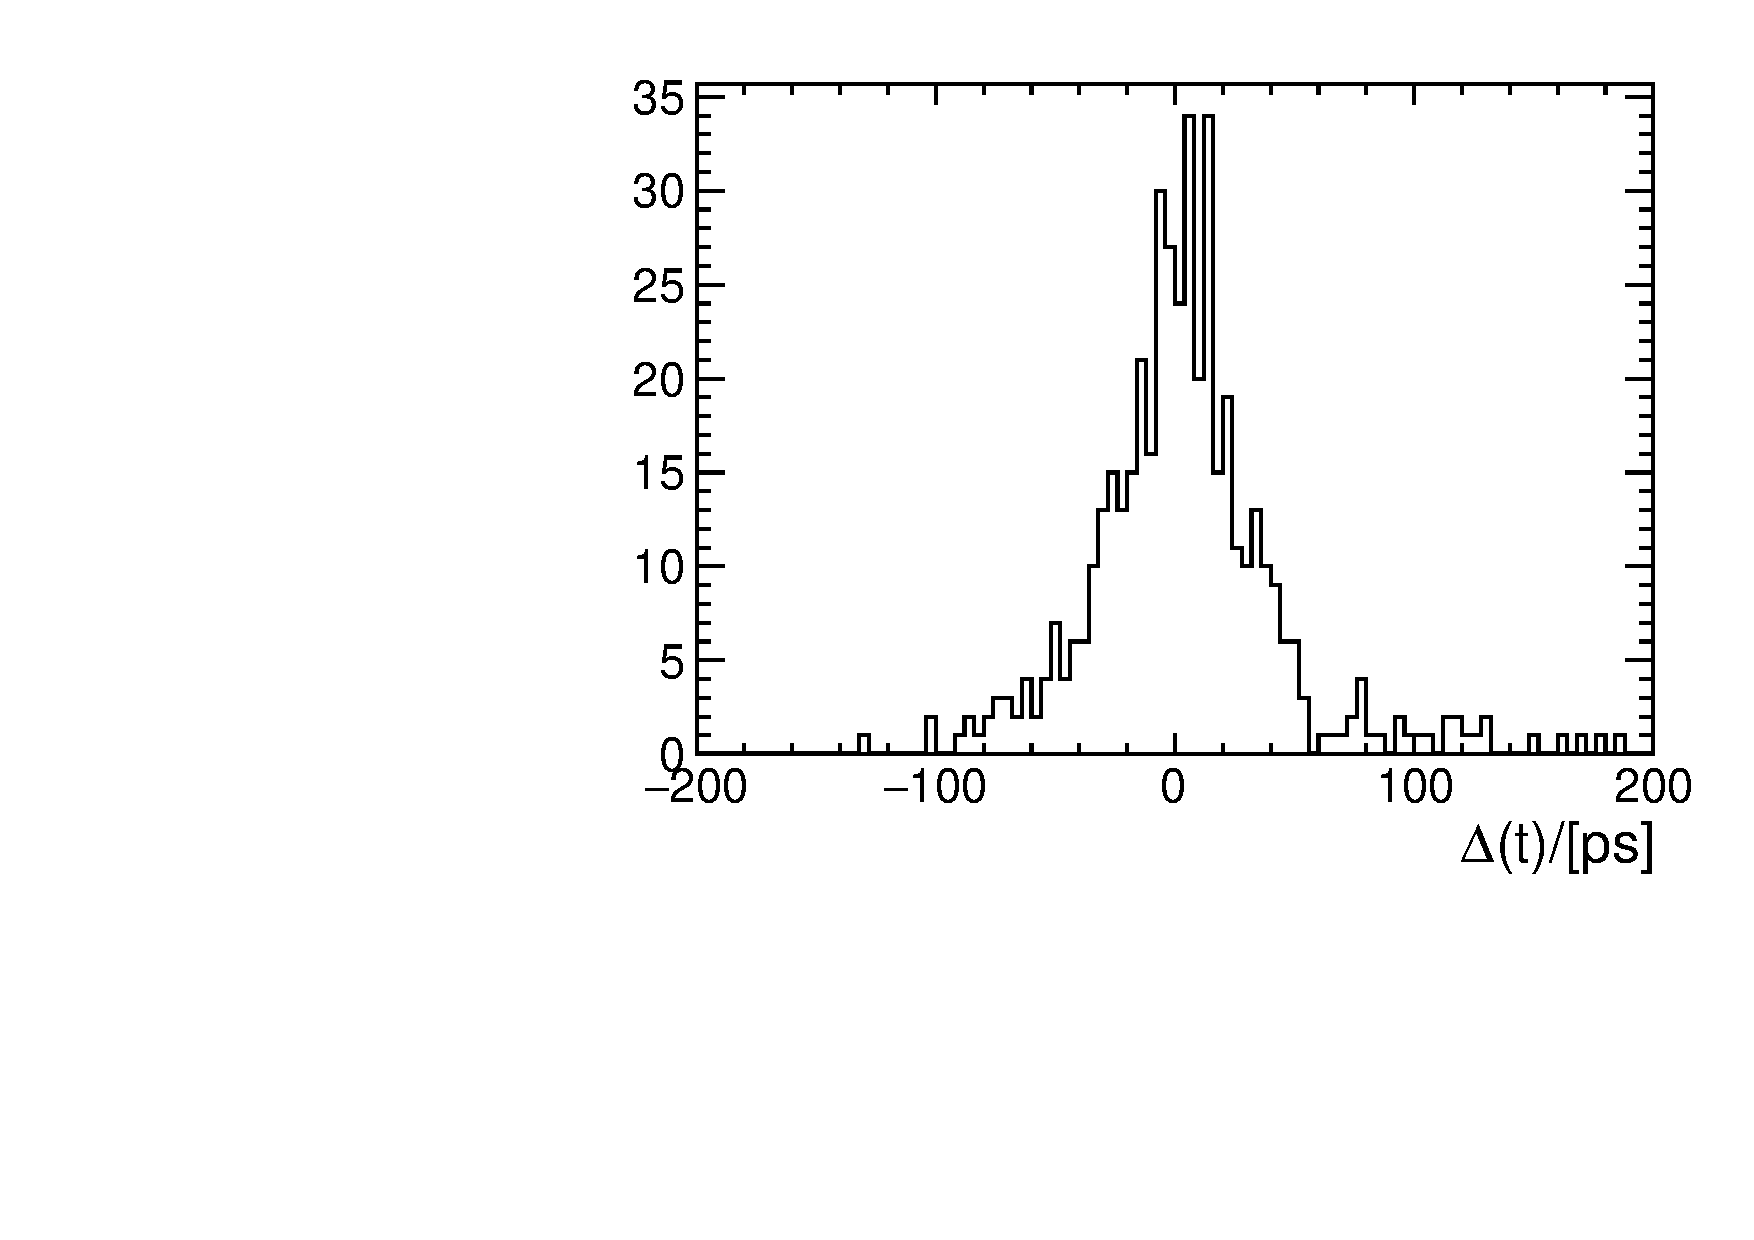
\includegraphics[width=0.49\linewidth]{Figures/06_ECAL/Brem/t_dis.pdf}
    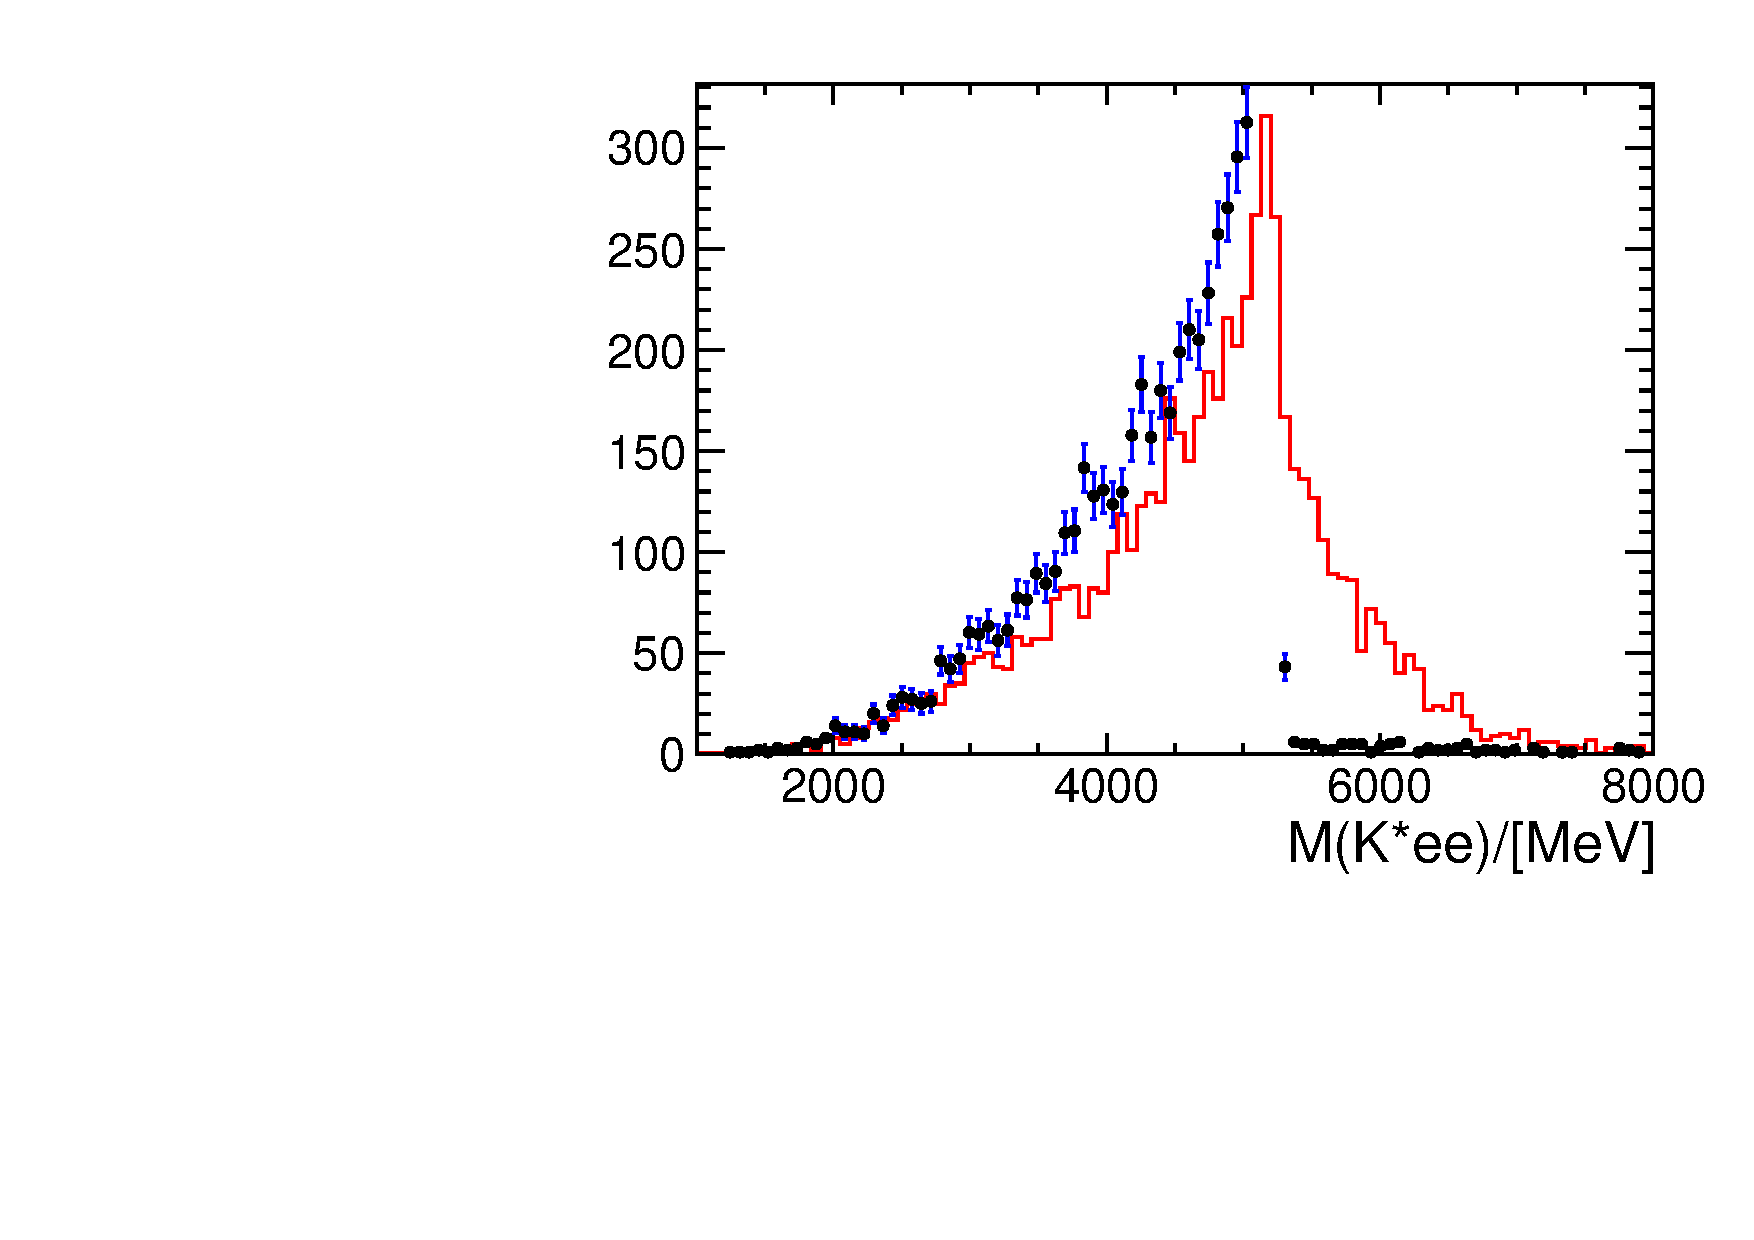
\includegraphics[width=0.49\linewidth]{Figures/06_ECAL/Brem/Bmass_compare.pdf}
    \vspace*{-0.5cm}
  \end{center}
  \caption{
      Left: the time difference between the electron and bremsstrahlung photon.
      Right: the $\Bd$ mass distribution before(blue point) or after bremsstrahlung recovery with time-matching included(red line).
  }
  \label{fig:Brem_B2kee}
\end{figure}
%%%%%%%%%%%%%%%%%%%%%%%%%%%%%%%%%%%%%%%%

The time difference between the electron and bremsstrahlung photon is shown in the left plot of Figure.~\ref{fig:Brem_B2kee},
we hope the time information can help improve the mass resolution of $\Bd$ reconstructed from $\Bd\to\Kstar\en\ep$ decay, 
the mass distribution is shown in the right plot of Figure.~\ref{fig:Brem_B2kee}.
However, 
there is no significant improvement for the invariant mass resolution of $\Kstar\ep\en$ when time information is used.

 









